% justify the Widom picture using the results from short solvent model
\documentclass[9pt]{article}
% Use the lineno option to display guide line numbers if required.
% Note that the use of elements such as single-column equations
% may affect the guide line number alignment. 
\usepackage{amsmath}
\usepackage{xcolor}
\usepackage{graphicx}

\renewcommand{\vec}[1]{\mbox{\boldmath$#1$}}

\newcommand{\erf}{\mathrm{erf}}
\newcommand{\erfc}{\mathrm{erfc}}
\newcommand{\me}{\mathrm{e}}

\newcommand{\mi}{\mathrm{i}}

\newcommand{\dif}{\mathrm{d}}

\newcommand{\pmf}{\emph{pmf\/}}

%\newcommand{\A}{\mathrm{\AA}}

\newcommand{\sAA}{_{\mathrm{ArAr}}}
\newcommand{\overbar}[1]{\mkern 1.5mu\overline{\mkern-1.5mu#1\mkern-1.5mu}\mkern 1.5mu}
%% jdw commands

\newcommand{\AZ}{\mathrm{A_{0}}}
\newcommand{\AR}{\mathrm{A_{R}}}
\newcommand{\A}{\mathrm{A}}
\newcommand{\R}{\mathrm{R}}
\newcommand{\M}{\mathrm{M}}
\newcommand{\W}{\mathrm{W}}
\newcommand{\MAR}{\mathrm{MA_{R}}}
\newcommand{\WAR}{\mathrm{WA_{R}}}
\newcommand{\MA}{\mathrm{MA}}
\newcommand{\ArAr}{\mathrm{ArAr}}
\newcommand{\WAr}{\mathrm{WAr}}
\newcommand{\WA}{\mathrm{WA}}
\newcommand{\B}{\mathrm{B}}
\newcommand{\XW}{\mathrm{XW}}
\newcommand{\HW}{\mathrm{HW}}
\newcommand{\OW}{\mathrm{OW}}
\newcommand{\Ion}{\mathrm{Ion}}
\newcommand{\Na}{\mathrm{Na}}
\newcommand{\Cl}{\mathrm{Cl}}
\newcommand{\Ca}{\mathrm{Ca}}

\newcommand{\Fl}{\mathrm{Fl}}
\newcommand{\f}{\mathrm{f}}
\newcommand{\fm}{\mathrm{fm}}
\newcommand{\sss}{\mathrm{ss}}
\newcommand{\scs}{\mathrm{sc}}
\newcommand{\capS}{\mathrm{S}}
\newcommand{\w}{\mathsf{w}}
\newcommand{\RN}{\mathbf{\overbar{R}}_N}
\newcommand{\Tr}{\mathrm{Tr}}

\begin{document}
\title{Justify Widom Picture}
\maketitle

In the PNAS paper, we defined the short solvent system. In the short solvent system, the solvent-solute and solvent-solvent coulomb interactions are truncated, and effective solute-solute interactions are introduced such that the solute-solute PMF of the short solvent system is the same as that of the full system. In this note, I want to define a different version of short solvent system, which I will denote as ``short solvent LJ system". In this short solvent LJ system, the coulomb interactions are kept intact. Instead the solute-solvent and solvent-solvent LJ attractions are truncated. Effective solute-solute interactions are introduced to counter the effects of the truncation.

In this short solvent LJ system, the solute-solute interaction has the following expression

\begin{align}
\begin{split}
 & \w_{\A\B}^{\sss}(r) =  \w_{\A\B}^{\f}(r) \\
+ & \frac{1}{2} \int d \vec{r}'\Big(\delta \rho_{\A}(\vec{r}_{\A}') + \delta \rho_{0, \A}(\vec{r}_{\A}')\Big) u_{1,\B\W}(r_{\B}') \\
 +&  \frac{1}{2} \int d \vec{r}'\Big( \delta \rho_{\B}(\vec{r}_{\B}') + \delta \rho_{0, \B}(\vec{r}_{\B}')\Big) u_{1,\A\W}(r_{\A}') \\
 + &  \frac{1}{2} \int \int d \vec{r}' d \vec{r}'' \Big( \delta \rho_{\A}(\vec{r}_{\A}') \delta \rho_{0, \B}(\vec{r}_{\B}'') \\
 + & \delta \rho_{\B}(\vec{r}_{\B}') \delta \rho_{0, \A}(\vec{r}_{\A}'') \Big) u_{1,\W\W}(|\vec{r}'' - \vec{r}'|) \,,
\end{split}
\label{eq:wss_finalfinal}
\end{align}
where $\w_{\A\B}^{\sss}(r)$ denotes the solute-solute interaction in the short solvent LJ system,  $\w_{\A\B}^{\f}(r)$ denotes the solute-solute interaction in the full system, $\delta \rho_{\A}(\vec{r}_{\A}') = \rho_{\A}(\vec{r}_{\A}') - \rho_b$ is the perturbation of water density by solute A in the full system, $\delta \rho_{0, \A}(\vec{r}_{\A}')$ is the perturbation of water density by solute A in the short solvent LJ system, $u_{1,\A\W}$ is the LJ attraction between solute $\A$ and solvent $\W$, and $u_{1,\W\W}$ is the LJ attraction between solvent $\W$. Eq.(\ref{eq:wss_finalfinal}) is an analogy of Eq.(17) of the PNAS paper.
%% write the equation 1.

Eq.(\ref{eq:wss_finalfinal}) can be connected to the Widom picture by making a simple approximation, which is assuming that the density of water outside the solute core is the bulk density, as shown in Fig \ref{fig:density}.
Under this approximation, we can show that  Eq.(\ref{eq:wss_finalfinal}) can be mapped to the Widom picture.
\begin{figure}[htp]
\centering
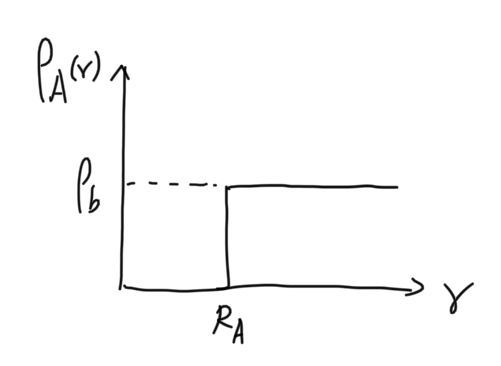
\includegraphics[scale=0.4]{Fig_density.png}
\caption{$\rho_{\A}(r)$ is the water density around solute A. $\rho_b$ is the bulk water density. $R_{\A}$ is the radius of the solute.}
\label{fig:density}
\end{figure}
%% key points of the widom picture

Under this approximation, we will have 
\begin{align}
\begin{split}
\delta \rho_{\A}(\vec{r}_{\A}') & = \delta \rho_{0, \A}(\vec{r}_{\A}')  = \delta \bar{\rho}_{\A} (\vec{r}_{\A}') \\
\delta \rho_{\B}(\vec{r}_{\B}') & = \delta \rho_{0, \B}(\vec{r}_{\B}')  =  \delta \bar{\rho}_{\B} (\vec{r}_{\B}')  \,,
\end{split}
\label{eq:approx}
\end{align}
where $\bar{\rho}$ denotes the step function shown in Fig \ref{fig:density}. Notice that  an effective hard sphere radius (e.g. $R_{\A}$ in Fig  \ref{fig:density}) needs to be chosen for the step function. In practice this effective radius is chosen such that the Kirkwood-Buff integral $\frac{1}{\rho_b}\int d\vec{r} \delta \bar{\rho}_{\A} (\vec{r}) $ is unchanged before and after the approximation.

Substitute Eq.(\ref{eq:approx}) into Eq.(\ref{eq:wss_finalfinal}), and we can get
\begin{align}
\begin{split}
 & \w_{\A\B}^{\sss}(r) =  \w_{\A\B}^{\f}(r) \\
+ & \int d \vec{r}'\delta \bar{\rho}_{\A}(\vec{r}_{\A}') u_{1,\B\W}(r_{\B}') \\
 +&  \int d \vec{r}'\delta \bar{\rho}_{\B}(\vec{r}_{\B}') u_{1,\A\W}(r_{\A}') \\
 + &  \frac{1}{2} \int \int d \vec{r}' d \vec{r}'' \Big( \delta \bar{\rho}_{\A}(\vec{r}_{\A}') \delta \bar{\rho}_{\B}(\vec{r}_{\B}'') \\
 + & \delta \bar{\rho}_{\B}(\vec{r}_{\B}') \delta \bar{\rho}_{\A}(\vec{r}_{\A}'') \Big) u_{1,\W\W}(|\vec{r}'' - \vec{r}'|) \,.
\end{split}
\label{eq:wss_finalfinalfinal}
\end{align}

The first two integrals in Eq.(\ref{eq:wss_finalfinalfinal}) is the contribution of solute-water attraction to the AB PMF. The corresponding integrands are non-zero only in the blue and red region of Fig \ref{fig:sw}. Making using of this property, the two integrals can be simplified to
 \begin{align}
\begin{split}
\mathrm{first\,\, two\,\, integrals\,\, of\,\, Eq.(\ref{eq:wss_finalfinalfinal})} & = -\int_{blue}d \vec{r}' \rho_b u_{1,\B\W}(r_{\B}')  -\int_{red}d \vec{r}' \rho_b u_{1,\A\W}(r_{\A}') \\
& = -n_{blue}\frac{\int_{blue}d \vec{r}' u_{1,\B\W}(r_{\B}')}{V_{blue}} -n_{red}\frac{\int_{red}d \vec{r}' u_{1,\A\W}(r_{\A}')}{V_{red}} \\
& = -n_{blue} \left\langle u_{1,\B\W} \right\rangle_{blue} - n_{red} \left\langle u_{1,\A\W} \right\rangle_{red}
\end{split}
\label{eq:wss_solutewater}
\end{align}
\begin{figure}[htp]
\centering
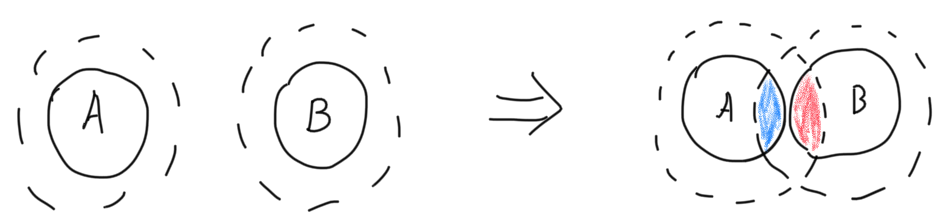
\includegraphics[scale=0.35]{Fig_SW.png}
\caption{The dashed curve around the solute stands for the range of solute-water attraction. When A and B associate, the water in the blue and red region are depleted to the bulk.}
\label{fig:sw}
\end{figure}

In Eq.(\ref{eq:wss_solutewater}) $n_{blue}$ and $n_{red}$ are the number of water molecules in the blue and red region that are depleted to the bulk upon the association of A and B. $\left\langle u_{1,\B\W} \right\rangle_{blue} = \frac{\int_{blue}d \vec{r}' u_{1,\B\W}(r_{\B}')}{V_{blue}} $ is the average strength of BW attraction in the blue region, where $V_{blue}$ is the volume of the blue region. $\left\langle u_{1,\A\W} \right\rangle_{red}$ is defined similarly.

The result of Eq.(\ref{eq:wss_solutewater}) is exactly what is predicted by Widom's picture. When the two solutes associated, the water in the blue and red region are depleted to the bulk, thus no longer subject to the solute-water attraction. The corresponding free energy change is just what is given by Eq.(\ref{eq:wss_solutewater}). 

The last integral of Eq.(\ref{eq:wss_finalfinalfinal}) is the contribution of water-water attraction, which can be further rewritten based on the renormalized part of LMF potential:
\begin{equation}
\mathrm{Last\,\, integral\,\, of\,\, Eq.(\ref{eq:wss_finalfinalfinal})} = \frac{1}{2}\int d \vec{r}'\delta \bar{\rho}_{\A}(\vec{r}_{\A}') \phi_{S, \B\W}(r_{\B}') +  \frac{1}{2} \int d \vec{r}'\delta \bar{\rho}_{\B}(\vec{r}_{\B}') \phi_{S,\A\W}(r_{\A}')
\label{eq:wss_ww}
\end{equation}
where $\phi_{S, \B\W}(r_{\B}') = \int d\vec{r}'' \delta \bar{\rho}_{ \B}(\vec{r}_{\B}'')u_{1,\W\W}(|\vec{r}'' - \vec{r}'|) $ is the renormalized part of LMF potential around solute B. $\phi_{S,\A\W}(r_{\A}')$ is defined similarly.

Note that the integrals in Eq.(\ref{eq:wss_ww}) are similar to the first two integrals of Eq.(\ref{eq:wss_finalfinalfinal}), with an additional prefactor $\frac{1}{2}$. We can connect Eq.(\ref{eq:wss_ww}) with Widom picture by following procedures analogous to what is shown in Eq.(\ref{eq:wss_solutewater}):
\begin{equation}
\mathrm{RHS\,\, of\,\, Eq.(\ref{eq:wss_ww})} = -\frac{1}{2} n_{green}  \left\langle \phi_{S,\B\W} \right\rangle_{green} - \frac{1}{2} n_{orange}  \left\langle \phi_{S,\A\W} \right\rangle_{orange}
\label{eq:wss_ww_simplified}
\end{equation}
where $n_{green}$ and $n_{orange}$ are the number of water molecules in the green and orange region that are depleted as shown in Fig \ref{fig:ww}. $\left\langle \phi_{S,\B\W} \right\rangle_{green}$ is the average strength of $\phi_{S,\B\W}$ in the green region. $\left\langle \phi_{S,\A\W} \right\rangle_{orange}$ is the average strength of $\phi_{S,\A\W}$ in the orange region.
\begin{figure}[htp]
\centering
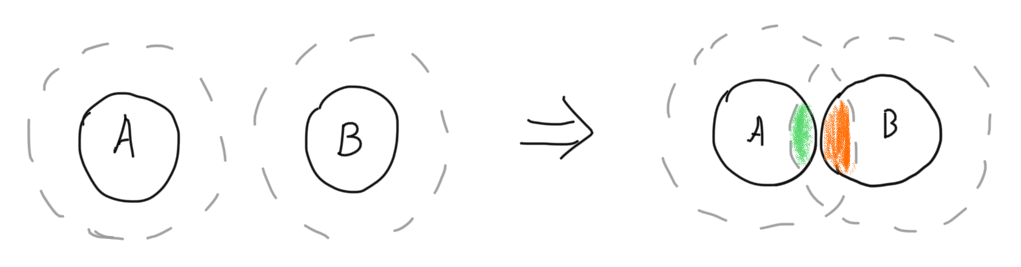
\includegraphics[scale=0.35]{Fig_WW.png}
\caption{The dashed curve around the solute stands for the range of $\phi_{S,\A\W}$ and $\phi_{S,\B\W}$ respectively. When A and B associate, the water in the green and orange region are depleted to the bulk.}
\label{fig:ww}
\end{figure}


Eq.(\ref{eq:wss_ww_simplified}) is consistent with Widom picture except for the $\frac{1}{2}$ prefactor. When the two solutes associate, the water in the green and orange region are depleted to the bulk, thus no longer subject to the renormalized part of LMF potential $\phi_{S, \B\W}$ and $\phi_{S,\A\W}$. Unlike the solute-water attraction $u_{1,\B\W}  $ and $u_{1,\A\W}$ which can be viewed as external field, $\phi_{S, \B\W}$ and $\phi_{S,\A\W}$ are effective potentials coming from solvent-solvent pair attractions. Remember that one needs an $\frac{1}{2}$ prefactor when calculating the energy coming from pair interactions. That's why the $\frac{1}{2}$ shows up in Eq.(\ref{eq:wss_ww_simplified}).

To summarize, under the approximation that the water density outside the solute core is the bulk density, the result in the short solvent paper can be rewritten as
 \begin{align}
\begin{split}
 \w_{\A\B}^{\sss}(r) =  \w_{\A\B}^{\f}(r)   & - n_{blue} \left\langle u_{1,\B\W} \right\rangle_{blue} - n_{red} \left\langle u_{1,\A\W} \right\rangle_{red} \\
  & - \frac{1}{2} n_{green}  \left\langle \phi_{S,\B\W} \right\rangle_{green} - \frac{1}{2} n_{orange}  \left\langle \phi_{S,\A\W} \right\rangle_{orange}  \,.
\end{split}
\label{eq:wss_finalfinalwidom}
\end{align}
The $\frac{1}{2}$ prefactor is due to the fact that $\phi_{S,\B\W} $ and $\phi_{S,\A\W}$ not an external field but  generated by solvent-solvent pair interactions. 
%% show equation 2 first
%% use a different notation, maybe \delta \bar{\rho}_A for the step function bulk density.

We verify the accuracy of Eq.(\ref{eq:wss_finalfinalwidom}) by studying the association of Argons in water. We performed MD simulation to obtain the contribution of Argon-water and water-water LJ attraction to the Argon-Argon PMF, and compared the simulation result to the LMF theory (Eq.(\ref{eq:wss_finalfinal})) and the Widom picture (Eq.(\ref{eq:wss_finalfinalwidom})).
The comparison is shown in Fig \ref{fig:pmf_ArAr}. As on can see, both LMF theory and Widom picture are pretty close to the simulation result. 

\begin{figure}[htp]
\centering
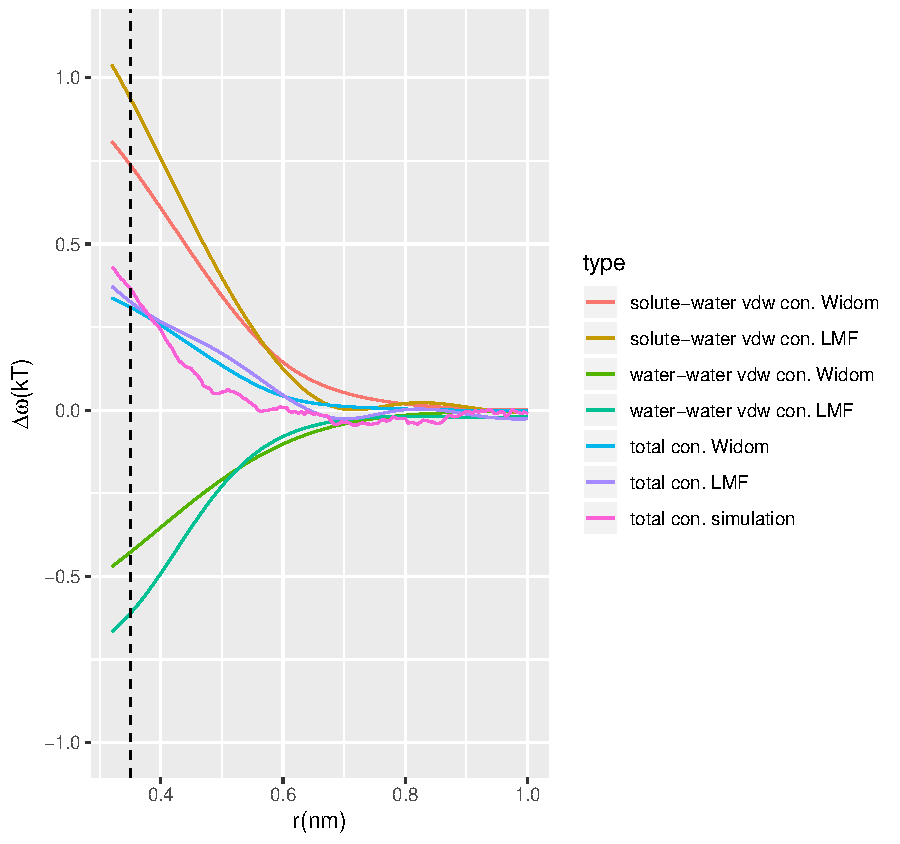
\includegraphics[scale=0.8]{widom_LMF_sim_ArAr.pdf}
\caption{The middle three curves  corresponds to the contribution of   Argon-water and water-water LJ attraction to the Argon-Argon PMF, obtained by simulation, LMF theory and Widom picture respectively. The top two curves correspond to the contribution of   Argon-water LJ attraction to the Argon-Argon PMF, obtained by LMF theory (first two integrals of Eq.(\ref{eq:wss_finalfinal})) and by Widom picture (first two integrals of Eq.(\ref{eq:wss_finalfinalwidom})) respectively. The bottom two curves correspond to the contribution of water-water LJ attraction to the Argon-Argon PMF, obtained by LMF theory (the last integral of Eq.(\ref{eq:wss_finalfinal})) and by Widom picture (the last integral of Eq.(\ref{eq:wss_finalfinalwidom})) respectively. }
\label{fig:pmf_ArAr}
\end{figure}
%% then just copy and paste

\end{document}
